%  FICHIER  :   template_fira_two_cols.tex
%  A copier à côté des autres .tex et à déclarer dans config.json
% ------------------------------------------------------------------
\documentclass[11pt,a4paper]{article}

% ─── pack de base ─────────────────────────────────────────────────
\usepackage[T1]{fontenc}
\usepackage[utf8]{inputenc}
\usepackage{textcomp}
\usepackage{newtxtext}
\usepackage[british]{babel}
\usepackage[left=0mm,right=0mm,top=0mm,bottom=0mm]{geometry}
\usepackage[stretch=25,shrink=25,tracking=true,letterspace=30]{microtype}
\usepackage{graphicx,xcolor,marvosym,enumitem,paracol,hyperref}
\usepackage{FiraSans}
\renewcommand{\familydefault}{\sfdefault}
\usepackage{array} 
\usepackage{tabularx}
\usepackage{ragged2e}
 \usepackage{fontawesome}
% ─── couleurs & listes ────────────────────────────────────────────
\definecolor{cvblue}{HTML}{304263}
\setlist{parsep=0pt,topsep=0pt,partopsep=1pt,itemsep=1pt,leftmargin=6mm}
\hypersetup{colorlinks=true,urlcolor=white,linkcolor=white}

% ─── macros maison (identiques au modèle original) ────────────────
\newcommand{\dates}[1]{\hfill\textbf{#1}}
\newcommand{\is}{\par\vskip.5ex plus .4ex}
\newcommand{\smaller}[1]{{\small$\diamond$\ #1}}
\newcommand{\headleft}[1]{\vspace*{3ex}\textsc{\textbf{#1}}\par%
  \vspace*{-1.5ex}\hrulefill\par\vspace*{0.7ex}}
\newcommand{\headright}[1]{\vspace*{2.5ex}\textsc{\Large\color{cvblue}#1}\par%
  \vspace*{-2ex}{\color{cvblue}\hrulefill}\par}

% ─── défaut de secours si sidetext absent dans d’autres modèles ───
\providecolor{sidetext}{rgb}{0,0,0}
\definecolor{maincolor}{HTML}{ffffff}
% ─────────────────────────── DOCUMENT ─────────────────────────────
\begin{document}
\thispagestyle{empty}
\setlength{\topskip}{0pt}\setlength{\parindent}{0pt}\setlength{\parskip}{0pt}
\raggedbottom

\begin{minipage}[t]{0.33\textwidth}
  % Bande bleue d’en-tête
  \colorbox{cvblue}{\begin{minipage}[t][5mm][t]{\textwidth}\null\end{minipage}}
  \vspace{-.2ex}
  \colorbox{cvblue!90}{%
    \color{white}\kern0.09\textwidth
    \begin{minipage}[t][293mm][t]{0.82\textwidth}\raggedright
      \vspace*{2.5ex}
      % -------- Identité ------------------------------------------
      \Large MOUROUVIN Judikael\normalsize

      % Photo (s’affiche seulement si af9c23b3d5d2496ebc2e43c55a5e46ad.png ≠ vide)
      \ifx\relaxaf9c23b3d5d2496ebc2e43c55a5e46ad.png\relax\else
        \vspace{2ex}\null\hfill
        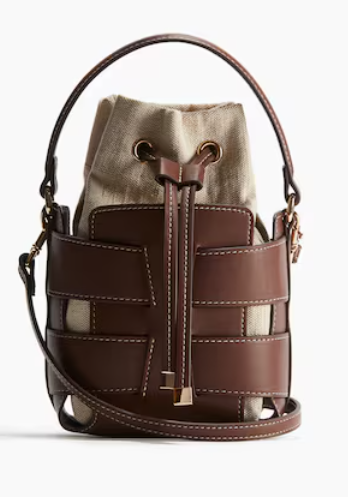
\includegraphics[width=0.2\textwidth]{af9c23b3d5d2496ebc2e43c55a5e46ad.png}
        \hfill\null
      \fi

      % -------- Profil -------------------------------------------
      \headleft{Profil}
      \begingroup           % ouvre un groupe local
         % rétablit la justification pleine
        Passionné d’informatique et de marketing numérique, je possède une double compétence en support technique, administration des systèmes et communication digitale. Mon alternance au sein de la DSI de la Mairie du Gosier m’a permis de piloter des projets digitaux, d’accompagner les utilisateurs et de contribuer à la stratégie numérique de la collectivité. Orienté résultats et doté d’un solide sens du service, je souhaite désormais rejoindre votre équipe à temps plein pour optimiser vos initiatives digitales.
      \endgroup             % referme : on revient à \raggedright

      % -------- Contact ------------------------------------------
      \headleft{Contact}\small
      \MVAt\  \texttt{jkmou971@gmail.com}\par
      \Mobilefone\ +590 0690 91 14 48\par
      \Letter\ Route de Cocoyer\par
      97190 Gosier\par
      \faLinkedin\  \href{}{}
      \normalsize

      % -------- Langues (si dispo) -------------------------------
      \ifx\relax\begin{itemize}[leftmargin=*]
\item English - \textcolor{gray}{}
\item Espagnol - \textcolor{gray}{}\end{itemize}\relax\else
        \headleft{Langues}
        \begin{itemize}[leftmargin=*]
\item English - \textcolor{gray}{}
\item Espagnol - \textcolor{gray}{}\end{itemize}
      \fi

      % -------- Compétences --------------------------------------
      \headleft{Compétences}
      \begin{itemize}[leftmargin=*]
\item Administration
\item Maintenance
\item Réseaux
\item Assistance
\item Diagnostic
\item Support
\item Configuration\end{itemize}

      % -------- Centres d’intérêt --------------------------------
      \headleft{Intérêts}
      \begin{itemize}[leftmargin=*]
\item Lecture
\item Sport
\item Musique
\item Voyage
\end{itemize}

    \end{minipage}\kern0.09\textwidth
  }
\end{minipage}
% ================================================================
\hskip2.5em
% ======================= COLONNE DROITE =========================
\begin{minipage}[t]{0.56\textwidth}
  \setlength{\parskip}{0.8ex}
  \vspace{2ex}

  % ---------- EXPERIENCE ----------------------------------------
  \headright{Expérience}
  \colorbox{maincolor}{%
  \begin{minipage}{\linewidth}
    \noindent
    \textbf{Alternant en marketing digital}\hfill 09/2023 - 08/2024\\
    Mairie du Gosier – DSI\\[-0.3em]
    \begin{itemize}[leftmargin=*]
      \item Pilotage de projets numériques, améliorant la coordination interne \item Analyse des besoins utilisateurs et déploiement de solutions adaptées, augmentant la satisfaction \item Support technique et formation des agents dans le cadre de la stratégie digitale
    \end{itemize}
  \end{minipage}}

\vspace{3mm}

\colorbox{maincolor}{%
  \begin{minipage}{\linewidth}
    \noindent
    \textbf{Animateur de la zone informatique}\hfill 09/2022 - 08/2023\\
    Pôle Emploi, Gosier\\[-0.3em]
    \begin{itemize}[leftmargin=*]
      \item Assistance et support technique aux utilisateurs, réduisant les interruptions de service \item Configuration et maintenance des postes de travail, garantissant la disponibilité du parc \item Diagnostic et résolution des incidents, améliorant la fiabilité du service
    \end{itemize}
  \end{minipage}}

\vspace{3mm}

\colorbox{maincolor}{%
  \begin{minipage}{\linewidth}
    \noindent
    \textbf{Stagiaire informaticien}\hfill 09/2020 - 06/2021\\
    Numerika, Baie-Mahault\\[-0.3em]
    \begin{itemize}[leftmargin=*]
      \item Installation et maintenance d’équipements informatiques, optimisant les performances \item Support de proximité aux utilisateurs, assurant la continuité des opérations
    \end{itemize}
  \end{minipage}}        % ← déjà formaté par build_placeholders()

  % ---------- EDUCATION -----------------------------------------
  \headright{Formation}
  \colorbox{maincolor}{%
  \begin{minipage}{\linewidth}
    \noindent
    \textbf{Bachelor Marketing Digital}\hfill 09/2023 - 08/2024\\
    CFA IUTS\\[-0.3em]
    \begin{itemize}[leftmargin=*]
      \item Stratégies de marketing en ligne, outils de communication digitale et analyse de performance
    \end{itemize}
  \end{minipage}}

\vspace{3mm}

\colorbox{maincolor}{%
  \begin{minipage}{\linewidth}
    \noindent
    \textbf{BTS Systèmes Numériques option Informatique et Réseaux}\hfill 09/2019 - 06/2021\\
    Lycée de Chevalier Saint Georges, Abymes\\[-0.3em]
    \begin{itemize}[leftmargin=*]
      \item Architecture réseau, administration systèmes et support technique
    \end{itemize}
  \end{minipage}}

\end{minipage}

\end{document}
